\chapter{Posicionamiento web}

El posicionamiento SEO es una disciplina que consiste en aplicar una serie de técnicas tanto dentro (On-Page) como fuera (Off-Page) de un determinado sitio Web, con el objetivo de optimizar y mejorar su visibilidad en los resultados orgánicos de los diferentes motores de búsqueda.

En otras palabras, es un conjunto de acciones enfocadas a mejorar las posiciones de las páginas de un sitio web en las listas de resultados de un buscador, para las consultas específicas de los diferentes usuarios, con el fin de aumentar su tráfico y las posibilidades de monetización.

Sin embargo, cabe preguntarse por qué es necesario el posicionamiento web. La razón es que cuanto más alta sea la posición de una página en la SERP (Search Engine Results Pages), en teoría, también mayor será el número de visitantes que llegarán a ella desde los diferentes motores de búsqueda. Por ejemplo, cuando un usuario escribe en Google la palabra clave «venta de pájaros Tenerife, el motor de búsqueda le presenta, en orden jerárquico, las páginas web que hablan sobre la venta de pájaros en la isla. En este caso, el usuario probablemente estará realizando una búsqueda para encontrar tiendas de pájaros en Tenerife.

Las tres palabras que habrá tecleado (venta, pájaros y Barcelona) son las que habrá utilizado Google para encontrar las páginas indexadas en su base de datos, que responden mejor a estas características y las habrá colocado en orden descendente según los parámetros específicos de sus algoritmos.

\section{¿Para qué sirve el SEO?}

Una vez que hemos comprendido qué es el SEO y cuál es su importancia dentro de una estrategia digital, a modo de resumen, podemos deducir que entre sus utilidades principales debemos discernir que nos beneficia por estos motivos:
\begin{itemize}
    \item Nos ayuda a mejorar nuestra visibilidad online. Al trabajar los diferentes factores que intervienen en el buen posicionamiento de nuestros contenidos, también por ende mejorará la visibilidad o cantidad de ocasiones en las que las distintas URL’s de nuestro dominio Web aparezca en los buscadores. De esta forma, dejaremos atrás la temida «invisibilidad» que nos puede diferenciar de otras Marcas más conocidas en nuestro sector.
    \item Captaremos más tráfico Web cualificado. Es muy importante que te deje claro en este punto lo de «cualificado», ya que si tenemos un negocio Online, no nos valdrá de nada atraer visitas provenientes de cualquier tipo de usuario.
    En otras palabras, suponiendo que tengo un eCommerce de venta de zapatillas deportivas, de nada nos vale atraer con nuestro contenidos a personas con un perfil «sedentario», ya que éstos presumiblemente no estarán interesados en comprarnos este producto.
    En cambio, si generamos artículos que ayuden a mejorar su día a día a deportistas y aficionados al running, por ejemplo, éstos sí estarán dentro del tipo de usuarios que potencialmente pudieran estar interesados en renovar sus zapatillas actuales.
    \item Incremento de las ventas. Derivado del motivo anterior, es evidente que, si atraigo una mayor cantidad de usuarios alineados con mi Buyer Persona, las ventas de mi tienda Online aumentarán, sino a corto, sí a medio/largo plazo. E igualmente ocurrirá si ofreces servicios…. Irás recibiendo cada vez mayor número de peticiones de presupuestos de posibles clientes.
    \item Mejorar nuestra reputación. A través de logres interiorizar qué es el SEO, lograremos que nuestra comunidad de seguidores y usuarios en general nos tengan en consideración y la imagen de Marca, tanto nuestra como la de nuestra empresa se incremente. Inevitablemente, la mejora de los 3 factores anteriores nos ayudará bastante en que se fomente el «boca a boca» y que nuestra Marca Personal y/o corporativa mejore paulatinamente.
\end{itemize}

\section{SEO OnPage}

La optimización OnPage consiste en todas aquellas acciones que se llevan a cabo dentro de la misma página, de forma que dependen en gran medida del administrador y no de terceros, como en el caso del OffPage. Se ocupa sobre todo de la adaptación de los contenidos, aunque los componentes estructurales y técnicos también juegan un papel importante. Los campos de acción más importantes del SEO OnPage:
\begin{itemize}
    \item Contenido: Nuestro objetivo es ofrecer información de gran valor, novedosa y relevante, lo que se llama contenido único en marketing (Unique Content). El contenido duplicado y el plagio de información no están permitidos, y el uso de palabras clave no debe exceder lo legible, pudiendo usar sinónimos. No hay que olvidar que los textos se dirigen a una persona, no exclusivamente al robot de Google.
    \item Estructura: Además de un buen contenido, elementos de formato como títulos, subtítulos, párrafos y listas aumentan la legibilidad de los artículos tanto para el usuario como para Google.
    \item Contenidos multimedia: Las imágenes, los vídeos y los gráficos son un medio ideal para enriquecer textos, pero para que Google los pueda “leer” es necesario que la palabra o las palabras claves también se encuentren en el nombre del archivo, en el título y en la descripción (Alt).
    \item Metadatos: Los también llamados Metatags comprenden información que los navegadores y los buscadores pueden interpretar. Los atributos más importantes para una optimización OnPage son el título y la descripción.
    \item Enlaces: Los links internos no solo ayudan a los usuarios a navegar por una página, sino también a Google. Cuando se trate de optimizar la estructura interna de enlaces es fundamental que el clickstream, o el recorrido que sigue un usuario y su registro, no sea muy largo.
    \item Programación: Otro aspecto a tener en cuenta es la optimización del código fuente, donde también se puede aplicar un diseño amigable para los buscadores: tiempos de carga excesivos, caídas o fallos en el código son señales fatales para Google.
\end{itemize}

\section{SEO OffPage}

La optimización OffPage comprende aquellas prácticas que afectan de manera indirecta a la página, es decir, que tienen lugar “fuera” de la página –al contrario que la OnPage, que tiene lugar en la misma web. Se pueden considerar como una especie de “señales” que apuntan a la página web desde el exterior y que Google interpreta como “votos de confianza”.

Cuando la página A enlaza a la página B, favorece a la reputación online de la página B, pues Google entiende que el contenido de esta página es especialmente relevante; la página B aumenta su autoridad y, por lo tanto, su posicionamiento. Los backlinks (enlaces entrantes) y menciones desde otras páginas o desde las redes sociales son, así, un factor muy importante a tener en cuenta a la hora de conseguir un buen puesto en la lista de resultados. Los campos de acción más importantes del SEO OffPage:
\begin{itemize}
    \item Linkbuilding. Los enlaces son uno de los factores de mayor peso a la hora de posicionar una página web, ya que sirven para medir el grado de estimación de una página. Es por esto que la creación de enlaces o linkbuilding concentra gran parte de los esfuerzos del SEO OffPage. Este concepto define el conjunto de medidas que se toman para generar enlaces entrantes (no se trata aquí de cantidad, sino de calidad) y lograr acuerdos con terceros por medio de diversas estrategias.
    \item Señales sociales. Este concepto se refiere a todos aquellos indicadores que proceden de redes sociales como Facebook, Twiter o Google+, aunque en algunos casos también puede incluir los comentarios en los blogs. Aunque no hay cifras oficiales que respalden la importancia de estas señales para el posicionamiento en los buscadores y las opiniones de los expertos son en este terreno dispares,  es un hecho que las señales positivas (el número de “Me gusta”, las veces que se comparte un contenido y los comentarios) no son del todo irrelevantes. Aquellas empresas que son activas en las redes sociales por medio de concursos, encuestas y otras estrategias, consiguen un aumento de la visibilidad, de las visitas cualificadas y del engagement del cliente.
\end{itemize}

\section{Herramientas para posicionamiento web}

\subsection{Ahrefs}

Esta «suite» tiene una gran variedad de funcionalidades que la hacen una gran ayuda para impulsar tus distintos proyectos. Si tuviese que destacar dos de sus puntos fuertes de Ahrefs, estos serían sin duda su capacidad para manejar  y analizar backlinks y la posibilidad de estudiar a la competencia a fondo.
Y es que, de entre todas sus funciones, Ahrefs es ampliamente conocida por ser una de las más potentes a la hora de rastrear y administrar los distintos backlinks que apuntan a tus páginas, así como también analizar la “salud” de cada uno, pudiendo evitar riesgos potenciales a tus sitios Web.

\begin{figure}[ht!]
    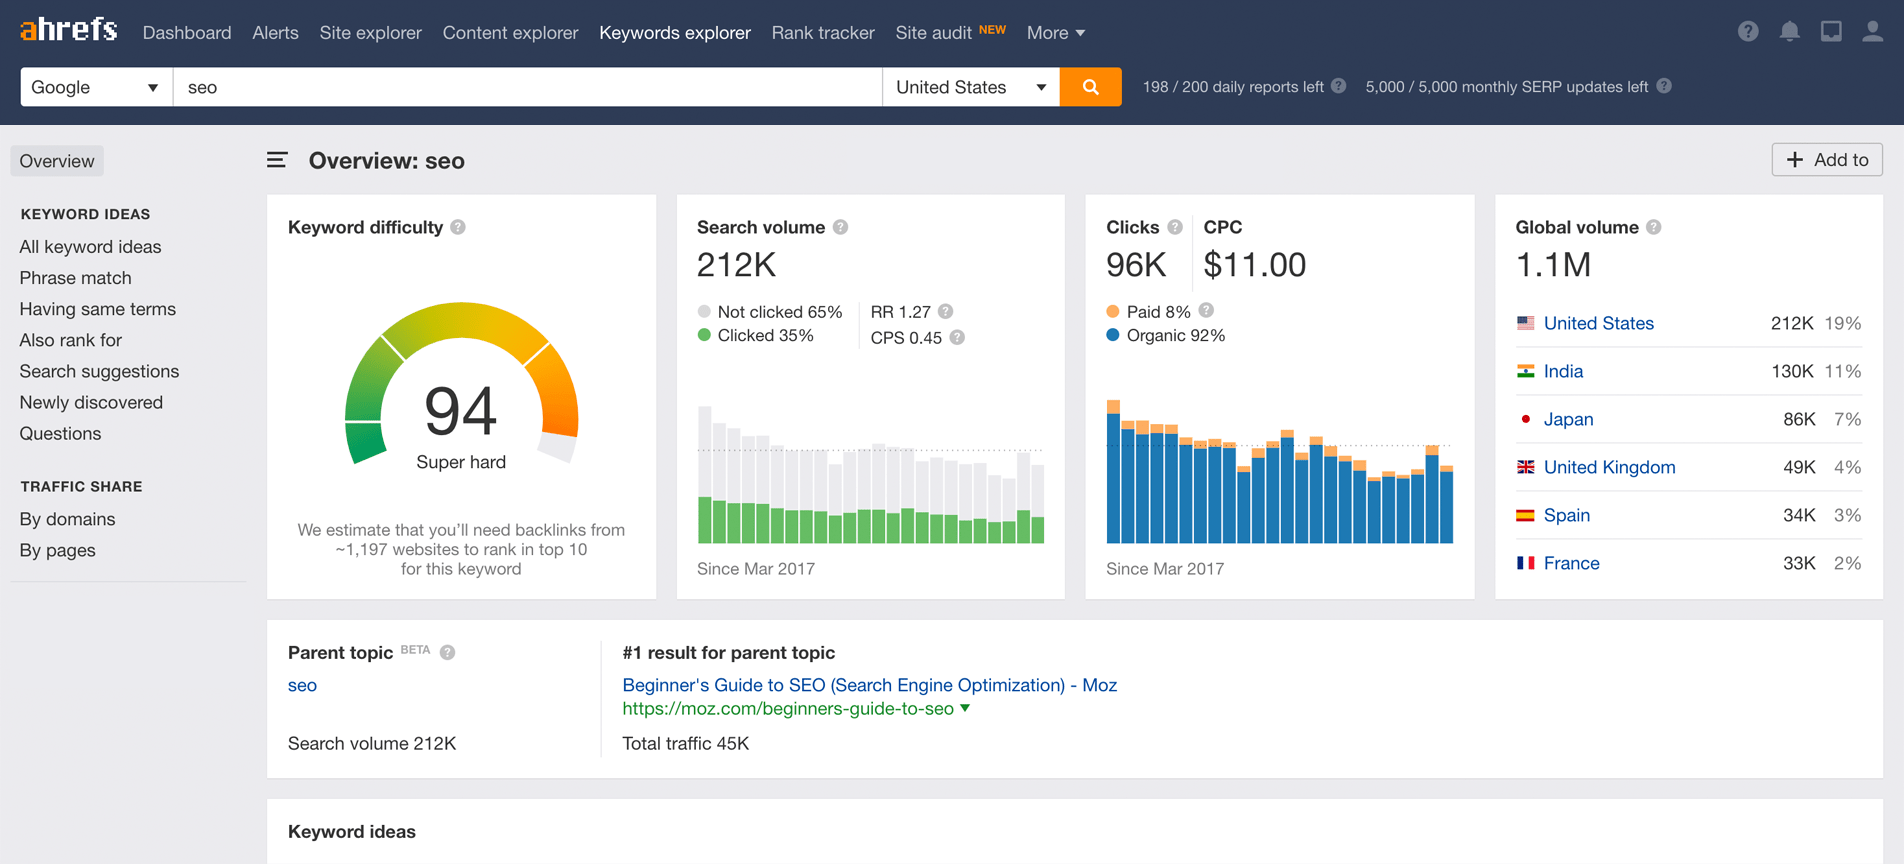
\includegraphics[width=\textwidth]{ahrefs.png}
    \caption{Ahrefs}
    \label{image-ahrefs}
\end{figure}

Por otro lado, ésta también pone a tu disposición diversas funciones que te ayudan estudiar a tu competencia, descubre las razones detrás del alto posicionamiento de tus competidores directos y desarrolla nuevas estrategias para superarlos. Ella te ofrece muchos datos y consejos para que puedas mejorar tu posicionamiento de forma óptima y así conseguir superar a tus competidores en el menor tiempo posible.

\subsection{SEMrush}

SEMrush ofrece a sus usuarios un catálogo de funcionalidades excepcionales, que no solo te permiten realizar análisis de Keywords, su principal función y la más desarrollada, sino que te ofrece la posibilidad de realizar un análisis de la competencia muy completo.

Si lo que deseas es encontrar las palabras claves adecuadas para enfocar tus contenidos, para tus campañas de Google Ads o para todo tu eCommerce, ésta es una de las mejores opciones.

\begin{figure}[ht!]
    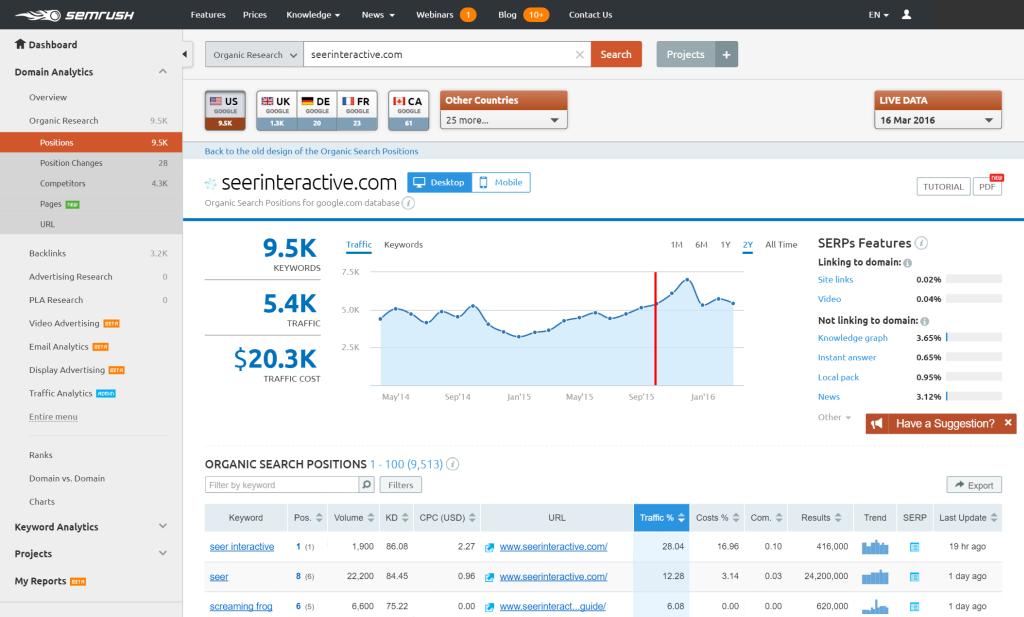
\includegraphics[width=\textwidth]{semrush.png}
    \caption{SemRush}
    \label{image-semrush}
\end{figure}

Cuenta con un enorme banco de datos de keywords que supera los 19 mil millones de términos, distribuidos en más de 140 países, ofreciendo a sus 5 millones de usuarios una precisión impecable a la hora de segmentar sus keywords.

Además, cuenta con un panel bastante completo que te permite analizar cada palabra clave y enlace hasta el más mínimo detalle.

\subsection{SE Ranking}

Otra de las herramientas SEO más populares que te podrás encontrar en Internet es sin duda SE Ranking, una potente «todo en uno» que te ofrece múltiples funcionalidades para optimizar tus proyectos y posicionar por encima de tus competidores.

Si bien ofrece múltiples funciones, destaca principalmente por la posibilidad de monitorear el posicionamiento de cada una de las palabras clave que tengas en él.

\begin{figure}[ht!]
    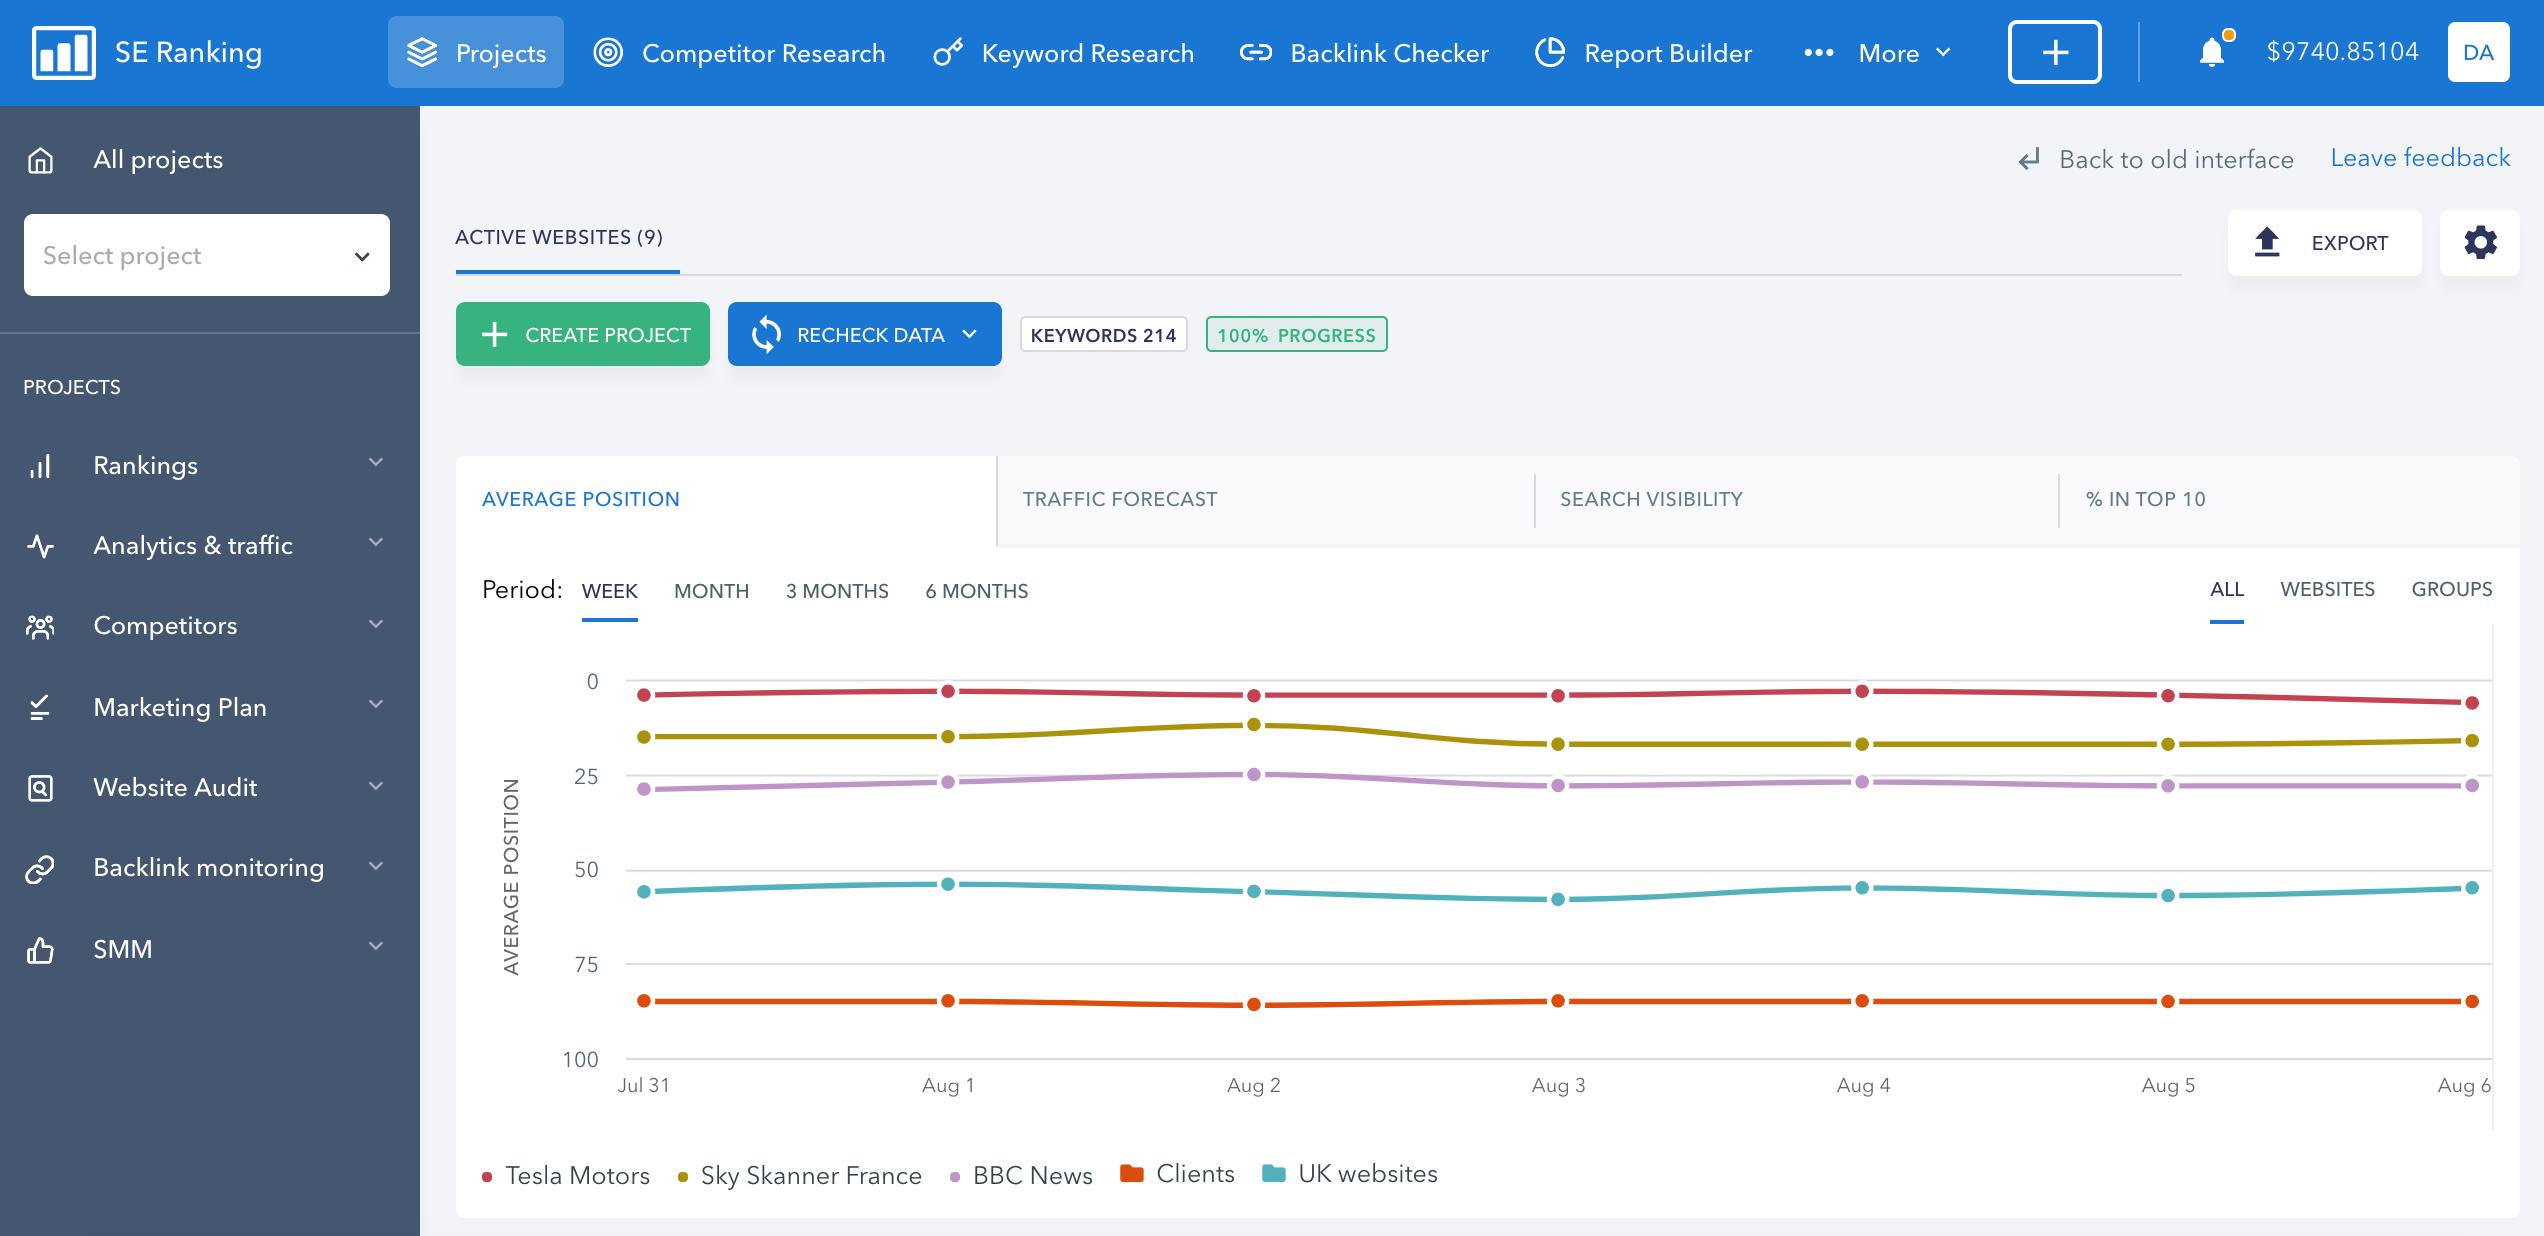
\includegraphics[width=\textwidth]{seranking.png}
    \caption{SE Ranking}
    \label{image-semrush}
\end{figure}

SERanking te ofrece la posibilidad de hacer una auditoría completa, e incluso la capacidad de comparar tu sitio con el de tu competencia directa.

Además, también cuenta con otras herramientas SEO como el agrupador de palabras clave, que te permite distribuir de manera eficiente las keywords que deseas utilizar en tu Web, así como también descubrir nuevos términos a utilizar.

Otra excelente ventaja es que te ayuda a planear tus campañas PPC de manera eficiente, basándose tanto en tu web como la de tu competencia.

\subsection{DinoRANK}

DinoRANK es una «suite SEO On-Page» en dónde encontrarás una gran variedad de herramientas que te permitirán monitorizar y optimizar el posicionamiento de tus proyectos desde un mismo lugar y a través de una interfaz bastante sencilla e intuitiva.

Bastante recomendable para profesionales freelancers que comienzan y/o para quien no disponga de demasiado presupuesto.

Ya sea que quieras realizar una auditoría a tu sitio web, analizar tu Pagerank interno o la salud de tu interlinking, o incluso si lo que quieres es encontrar nuevas palabras claves para tus contenidos, con DinoRANK podrás hacerlo.

\begin{figure}[ht!]
    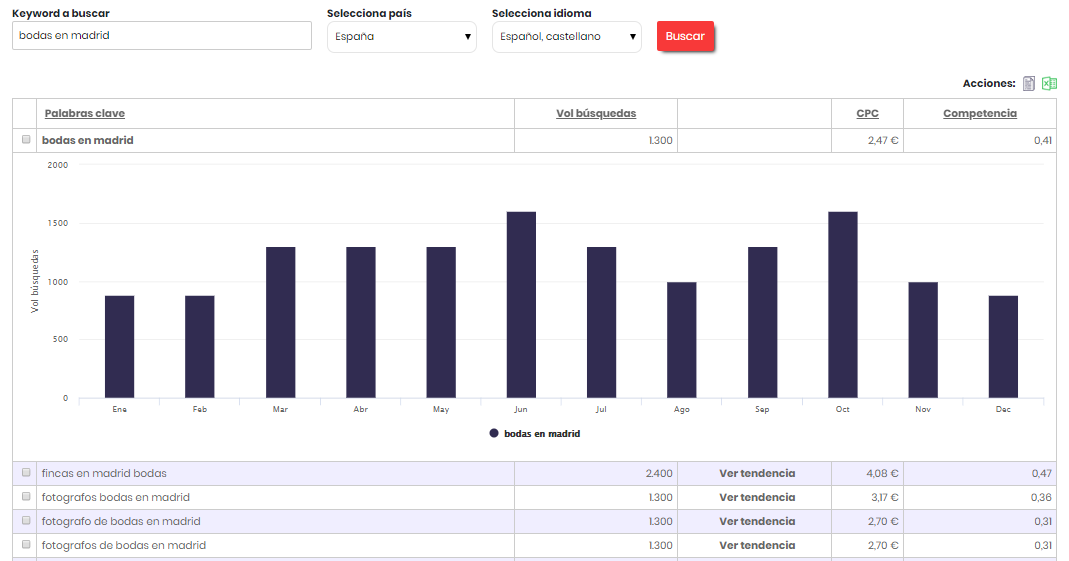
\includegraphics[width=\textwidth]{dinorank.png}
    \caption{DinoRANK}
    \label{image-dinorank}
\end{figure}

Las diversas posibilidades que ofrece y su bajo costo hacen de esta una de las mejores herramientas SEO para principiantes. Además, para aprender a usarla, puedes también consultar este tutorial completo de Dinorank, en él te enseño todo lo que necesitas saber.

\subsection{Screaming Frog}

El SEO On-Page es un factor determinante para el correcto posicionamiento de un sitio Web y saber optimizarlo puede volverse crucial para que tu proyecto tenga el éxito deseado. Sin embargo, para poder trabajarlo y optimizarlo, se hace necesario conocer el estado actual de tu sitio, y para lograrlo, una de las herramientas SEO que puedes utilizar y que personalmente te recomiendo es ésta.

\begin{figure}[ht!]
    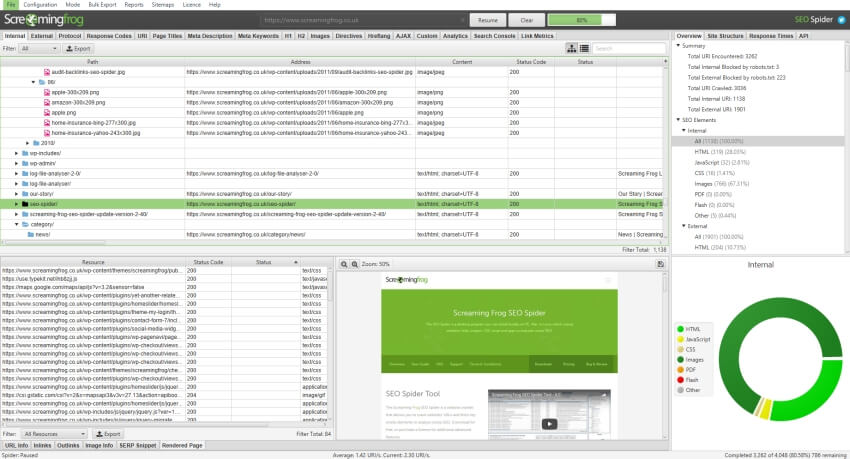
\includegraphics[width=\textwidth]{screaming-frog.jpg}
    \caption{Screaming Frog}
    \label{image-screaming-frog}
\end{figure}

Screaming Frog es un «crawler», que ingresa a tu URL y extrae en tiempo real toda la información relacionada con tu SEO On-Page, permitiéndote obtener datos importantes como posibles errores de redirección, fallos en meta títulos y meta descripciones, tu Sitemap, la estructura de tus enlaces, entre muchas cosas más.

Lo mejor de todo es que esta herramienta es capaz de analizar tu dominio completo en profundidad, sin importar si se trata de un Blog pequeño o de una enorme tienda Online.

Te informa en tiempo real de la situación actual del site, para que tu puedas detectar cualquier inconveniente que pueda estar afectando el rendimiento de tu proyecto.